% Compile from the manuscript root:
% latexmk -pdf -outdir=.verification/mixed-figures figures/MixedW.tex
% Copy the resulting MixedW.pdf beside this source for inclusion in main.tex.
\documentclass[tikz,border=4pt,11pt]{standalone}
\usepackage[T1]{fontenc}
\usepackage{lmodern}
\usepackage{amsmath}
\usetikzlibrary{arrows.meta}

\begin{document}
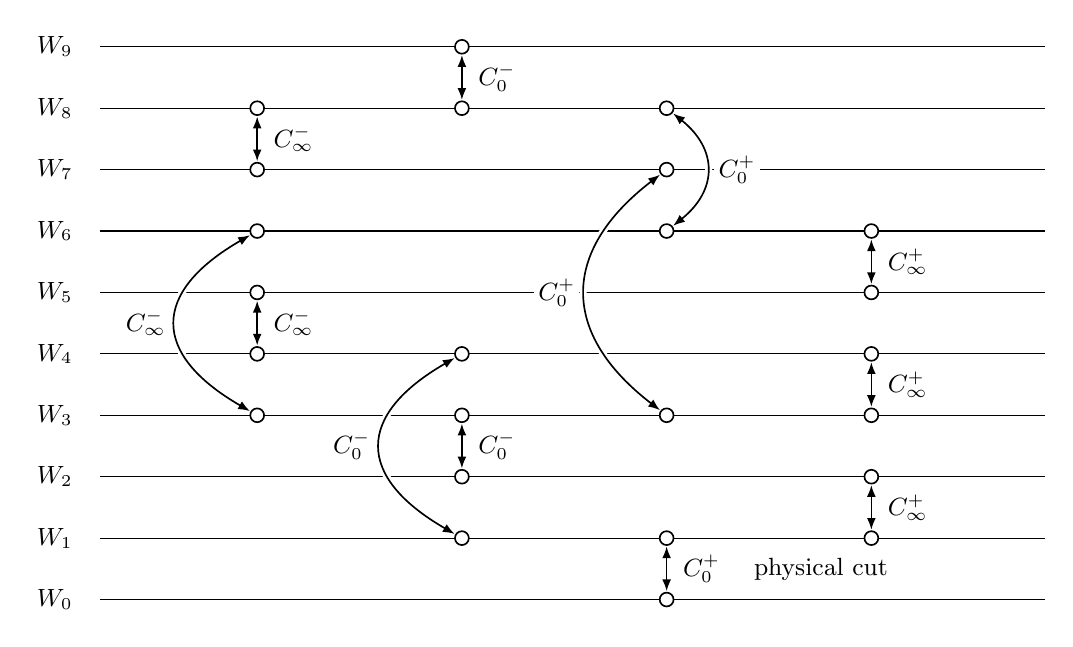
\begin{tikzpicture}[
    x=1cm,y=.78cm,font=\small,
    sheet/.style={line width=.45pt},
    exchange/.style={line width=.6pt,{Latex[length=1.5mm]}-{Latex[length=1.5mm]},
        shorten <=3pt,shorten >=3pt,preaction={draw=white,line width=2.5pt}},
    endpoint/.style={circle,draw,line width=.6pt,fill=white,inner sep=0pt,
        minimum size=5pt},
    cut label/.style={fill=white,inner sep=1.5pt}
]
    % Numeric row order uses the current Appendix A.5 labels, including 7 and 8.
    \foreach \index in {0,...,9} {
        \draw[sheet] (0,\index) -- (12,\index);
        \node[anchor=east] at (-.22,\index) {$W_{\index}$};
    }

    % W exchange: C_infty^- (3,6), (4,5), (7,8).
    \draw[exchange] (2,3) .. controls (.65,4) and (.65,5) .. (2,6);
    \node[cut label,anchor=east] at (.9,4.5) {$C_\infty^-$};
    \draw[exchange] (2,4) -- (2,5);
    \node[cut label,anchor=west] at (2.15,4.5) {$C_\infty^-$};
    \draw[exchange] (2,7) -- (2,8);
    \node[cut label,anchor=west] at (2.15,7.5) {$C_\infty^-$};

    % W exchange: C_0^- (1,4), (2,3), (8,9).
    \draw[exchange] (4.6,1) .. controls (3.25,2) and (3.25,3) .. (4.6,4);
    \node[cut label,anchor=east] at (3.5,2.5) {$C_0^-$};
    \draw[exchange] (4.6,2) -- (4.6,3);
    \node[cut label,anchor=west] at (4.75,2.5) {$C_0^-$};
    \draw[exchange] (4.6,8) -- (4.6,9);
    \node[cut label,anchor=west] at (4.75,8.5) {$C_0^-$};

    % W exchange: C_0^+ (0,1), (3,7), (6,8).
    \draw[exchange] (7.2,0) -- (7.2,1);
    \node[cut label,anchor=west] at (7.35,.5) {$C_0^+$};
    \node[cut label,anchor=west] at (8.25,.5) {physical cut};
    \draw[exchange] (7.2,3) .. controls (5.85,4.33) and (5.85,5.67) .. (7.2,7);
    \node[cut label,anchor=east] at (6.1,5) {$C_0^+$};
    \draw[exchange] (7.2,6) .. controls (7.85,6.67) and (7.85,7.33) .. (7.2,8);
    \node[cut label,anchor=west] at (7.8,7) {$C_0^+$};

    % W exchange: C_infty^+ (1,2), (3,4), (5,6).
    \foreach \lower/\upper in {1/2,3/4,5/6} {
        \draw[exchange] (9.8,\lower) -- (9.8,\upper);
        \node[cut label,anchor=west] at (9.95,{(\lower+\upper)/2}) {$C_\infty^+$};
    }

    \foreach \x/\y in {
        2/3,2/6,2/4,2/5,2/7,2/8,
        4.6/1,4.6/4,4.6/2,4.6/3,4.6/8,4.6/9,
        7.2/0,7.2/1,7.2/3,7.2/7,7.2/6,7.2/8,
        9.8/1,9.8/2,9.8/3,9.8/4,9.8/5,9.8/6
    }
        \node[endpoint] at (\x,\y) {};
\end{tikzpicture}
\end{document}
